\chapter{Dynamic Programming}

\section{Convex Hull Trick}

    If multiple transitions of the DP can be seen as 
    first degree polynomials (lines). CHT can be used to optimized it

    Some valid functions:

    $ax + b$
    
    $cx^2 + ax + b$ 
    (ignore $cx^2$ if c is independent)

    \kactlimport{cht-dynamic.cpp}

\section{Li-chao Tree}

    Works for any type of function that has the \textbf{transcending property}:

    Given two functions f(x),g(x) of that type, 
    if f(t) is greater than/smaller than g(t) for some x=t,
    then f(x) will be greater than/smaller than g(x) for x>t.
    In other words, once f(x) “win/lose” g(x), f(x) will continue to “win/lose” g(x).

    The most common one is the line function: $ ax + b $

\section{SOS DP}

    \textbf{Sum over Subsets DP (SOS DP)} computes how many elements there are for each mask
    which are a subset of this mask.

    This can be modified for other operations in which the subset contributes for the mask
    .
    \textit{Example:}

    \textbf{10}0\textbf{1} if a subset of \textbf{11}0\textbf{1};

    \textbf{00}0\textbf{1} if a subset of \textbf{11}0\textbf{1};
    
    \textbf{11}0\textbf{0} if a subset of \textbf{11}0\textbf{1};
    
    \textbf{11}0\textbf{1} if a subset of \textbf{11}0\textbf{1};

    \begin{center}
        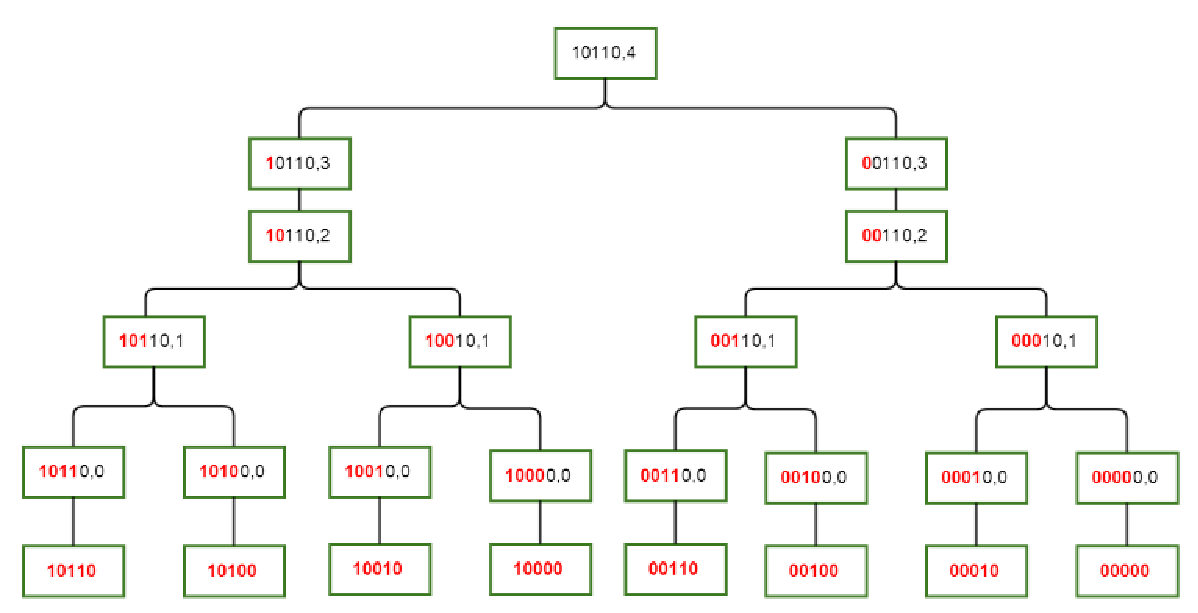
\includegraphics[width=9cm]{content/dynamic-programming/sos-example.pdf}
    \end{center}

    \kactlimport{sos-dp.cpp}